\chapter{Monodromy groups of rank 4}

\section{Deux 4-transpositions}

\subsection{Aucun carré}

\subsubsection{Longueur 8}

\begin{figure}[H]
  \begin{center}
    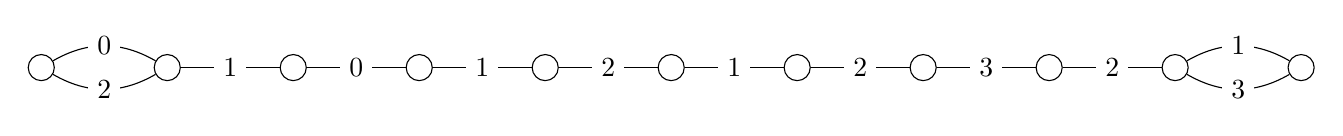
\begin{tikzpicture}[scale=.8]

      \begin{scope}[every node/.style={circle,draw}]
        \node (1)  at (0,0) {};
        \node (2)  at (2,0) {};
        \node (3)  at (4,0) {};
        \node (4)  at (6,0)  {};
        \node (5)  at (8,0)  {};
        \node (6)  at (10,0)  {};
        \node (7)  at (12,0)  {};
        \node (8)  at (18,0)  {};
        \node (9)  at (20,0)  {};
        \node (10) at (16,0)  {};
        \node (11) at (14,0)  {};
      \end{scope}

      \begin{scope}[every node/.style={fill=white}]

        \begin{scope}[every edge/.style={draw}]
          \path (1)  edge[bend left=30] node {$0$} (2);
          \path (3)  edge node {$0$} (4);
          \path (2)  edge node {$1$} (3);
          \path (4)  edge node {$1$} (5);
          \path (6)  edge node {$1$} (7);
          \path (8)  edge[bend left=30] node {$1$} (9);
          \path (1)  edge[bend right=30] node {$2$} (2);
          \path (5)  edge node {$2$} (6);
          \path (7)  edge node {$2$} (11);
          \path (8)  edge node {$2$} (10);
          \path (8)  edge[bend right=30] node {$3$} (9);
          \path (10) edge node {$3$} (11);
        \end{scope}
      \end{scope}

    \end{tikzpicture}
    \caption{[1, 995, 2703, 234]}
  \end{center}
\end{figure}

\begin{figure}[H]
  \begin{center}
    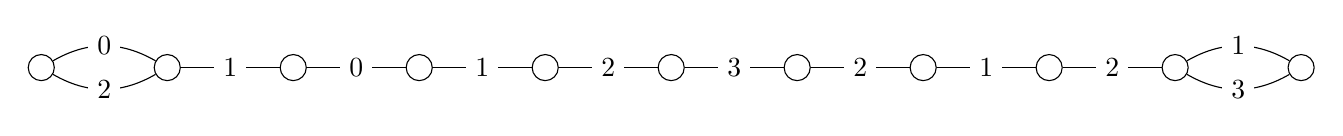
\begin{tikzpicture}[scale=.8]

      \begin{scope}[every node/.style={circle,draw}]
        \node (1)  at (0,0) {};
        \node (2)  at (2,0) {};
        \node (3)  at (4,0) {};
        \node (4)  at (6,0)  {};
        \node (5)  at (8,0)  {};
        \node (6)  at (20,0)  {};
        \node (7)  at (18,0)  {};
        \node (8)  at (16,0)  {};
        \node (9)  at (14,0)  {};
        \node (10) at (10,0)  {};
        \node (11) at (12,0)  {};
      \end{scope}

      \begin{scope}[every node/.style={fill=white}]

        \begin{scope}[every edge/.style={draw}]
          \path (1)  edge[bend left=30] node {$0$} (2);
          \path (3)  edge node {$0$} (4);
          \path (2)  edge node {$1$} (3);
          \path (4)  edge node {$1$} (5);
          \path (6)  edge[bend right=30] node {$1$} (7);
          \path (8)  edge node {$1$} (9);
          \path (1)  edge[bend right=30] node {$2$} (2);
          \path (5)  edge node {$2$} (10);
          \path (7)  edge node {$2$} (8);
          \path (9)  edge node {$2$} (11);
          \path (6)  edge[bend left=30] node {$3$} (7);
          \path (10) edge node {$3$} (11);
        \end{scope}
      \end{scope}

    \end{tikzpicture}
    \caption{[1, 995, 5928, 219]}
  \end{center}
\end{figure}

\begin{figure}[H]
  \begin{center}
    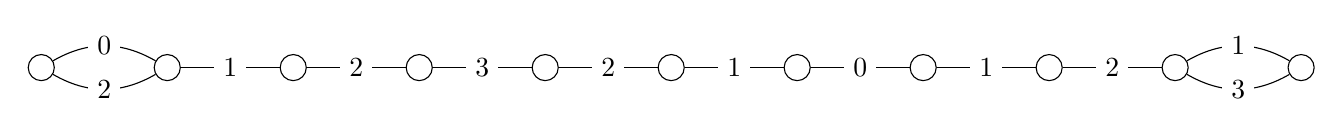
\begin{tikzpicture}[scale=.8]

      \begin{scope}[every node/.style={circle,draw}]
        \node (1)  at (14,0) {};
        \node (2)  at (12,0)  {};
        \node (3)  at (2,0)  {};
        \node (4)  at (0,0)  {};
        \node (5)  at (6,0)  {};
        \node (6)  at (8,0)  {};
        \node (7)  at (10,0)  {};
        \node (8)  at (16,0)  {};
        \node (9)  at (18,0)  {};
        \node (10) at (20,0)  {};
        \node (11) at (4,0) {};
      \end{scope}

      \begin{scope}[every node/.style={fill=white}]

        \begin{scope}[every edge/.style={draw}]
          \path (1)  edge node {$0$} (2);
          \path (3)  edge[bend right=30] node {$0$} (4);
          \path (1)  edge node {$1$} (8);
          \path (2)  edge node {$1$} (7);
          \path (3)  edge node {$1$} (11);
          \path (9)  edge[bend left=30] node {$1$} (10);
          \path (3)  edge[bend left=30] node {$2$} (4);
          \path (5)  edge node {$2$} (11);
          \path (6)  edge node {$2$} (7);
          \path (8)  edge node {$2$} (9);
          \path (5)  edge node {$3$} (6);
          \path (9)  edge[bend right=30] node {$3$} (10);
        \end{scope}
      \end{scope}

    \end{tikzpicture}
    \caption{[1, 1029, 3875, 147]}
  \end{center}
\end{figure}

\subsubsection{Longueur 6}

\begin{figure}[H]
  \begin{center}
    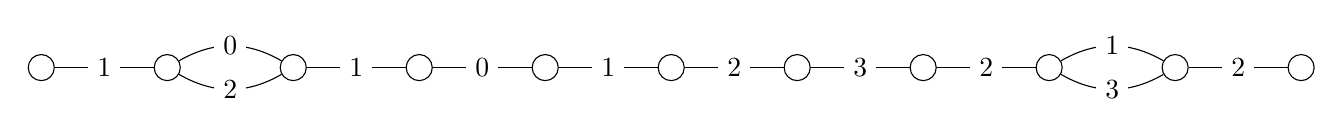
\begin{tikzpicture}[scale=.8]

      \begin{scope}[every node/.style={circle,draw}]
        \node (1)  at (2,0)  {};
        \node (2)  at (4,0)  {};
        \node (3)  at (6,0)  {};
        \node (4)  at (8,0)  {};
        \node (5)  at (10,0)  {};
        \node (6)  at (12,0)  {};
        \node (7)  at (14,0)  {};
        \node (8)  at (20,0) {};
        \node (9)  at (18,0)  {};
        \node (10) at (16,0) {};
        \node (11) at (0,0) {};
      \end{scope}

      \begin{scope}[every node/.style={fill=white}]

        \begin{scope}[every edge/.style={draw}]
          \path (1)  edge[bend left=30] node {$0$} (2);
          \path (3)  edge node {$0$} (4);
          \path (1)  edge node {$1$} (11);
          \path (2)  edge node {$1$} (3);
          \path (4)  edge node {$1$} (5);
          \path (9)  edge[bend right=30] node {$1$} (10);
          \path (1)  edge[bend right=30] node {$2$} (2);
          \path (5)  edge node {$2$} (6);
          \path (7)  edge node {$2$} (10);
          \path (8)  edge node {$2$} (9);
          \path (6)  edge node {$3$} (7);
          \path (9)  edge[bend left=30] node {$3$} (10);
        \end{scope}
      \end{scope}

    \end{tikzpicture}
    \caption{[1, 1075, 4159, 153]}
  \end{center}
\end{figure}


\begin{figure}[H]
  \begin{center}
    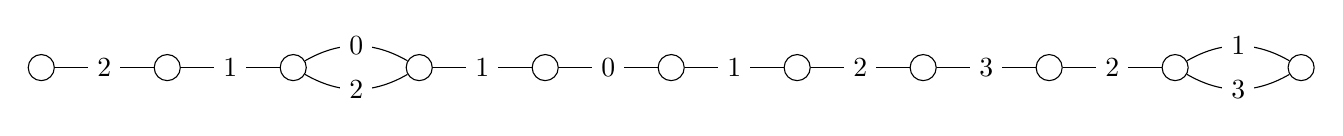
\begin{tikzpicture}[scale=.8]

      \begin{scope}[every node/.style={circle,draw}]
        \node (1)  at (10,0)  {};
        \node (2)  at (8,0)  {};
        \node (3)  at (6,0)  {};
        \node (4)  at (4,0)  {};
        \node (5)  at (2,0) {};
        \node (6)  at (0,0)  {};
        \node (7)  at (14,0) {};
        \node (8)  at (16,0)  {};
        \node (9)  at (20,0)  {};
        \node (10) at (18,0) {};
        \node (11) at (12,0) {};
      \end{scope}

      \begin{scope}[every node/.style={fill=white}]

        \begin{scope}[every edge/.style={draw}]
          \path (1)  edge node {$0$} (2);
          \path (3)  edge[bend right=30] node {$0$} (4);
          \path (1)  edge node {$1$} (11);
          \path (2)  edge node {$1$} (3);
          \path (4)  edge node {$1$} (5);
          \path (9)  edge[bend right=30] node {$1$} (10);
          \path (3)  edge[bend left=30] node {$2$} (4);
          \path (5)  edge node {$2$} (6);
          \path (7)  edge node {$2$} (11);
          \path (8)  edge node {$2$} (10);
          \path (7)  edge node {$3$} (8);
          \path (9)  edge[bend left=30] node {$3$} (10);
        \end{scope}
      \end{scope}

    \end{tikzpicture}
    \caption{[1, 1075, 1579, 160]}
  \end{center}
\end{figure}

\begin{figure}[H]
  \begin{center}
    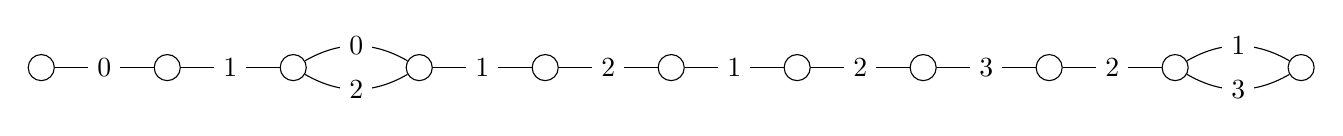
\begin{tikzpicture}[scale=.8]

      \begin{scope}[every node/.style={circle,draw}]
        \node (1)  at (20,0) {};
        \node (2)  at (18,0) {};
        \node (3)  at (16,0) {};
        \node (4)  at (14,0)  {};
        \node (5)  at (12,0)  {};
        \node (6)  at (10,0)  {};
        \node (7)  at (8,0)  {};
        \node (8)  at (6,0)  {};
        \node (9)  at (4,0)  {};
        \node (10) at (2,0)  {};
        \node (11) at (0,0)  {};
      \end{scope}

      \begin{scope}[every node/.style={fill=white}]

        \begin{scope}[every edge/.style={draw}]
          \path (1)  edge[bend left=30] node {$3$} (2);
          \path (3)  edge node {$3$} (4);
          \path (2)  edge node {$2$} (3);
          \path (4)  edge node {$2$} (5);
          \path (6)  edge node {$2$} (7);
          \path (8)  edge[bend left=30] node {$2$} (9);
          \path (1)  edge[bend right=30] node {$1$} (2);
          \path (5)  edge node {$1$} (6);
          \path (7)  edge node {$1$} (8);
          \path (9)  edge node {$1$} (10);
          \path (8)  edge[bend right=30] node {$0$} (9);
          \path (10) edge node {$0$} (11);
        \end{scope}
      \end{scope}

    \end{tikzpicture}
    \caption{[1, 995, 994, 234]}
  \end{center}
\end{figure}

\begin{figure}[H]
  \begin{center}
    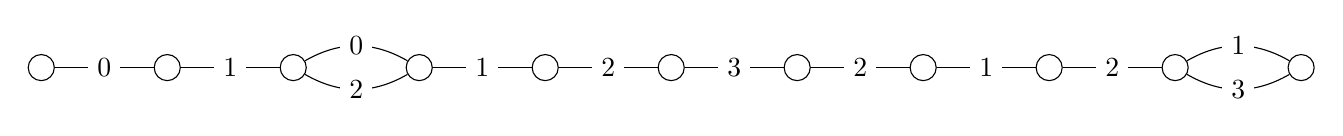
\begin{tikzpicture}[scale=.8]

      \begin{scope}[every node/.style={circle,draw}]
        \node (1)  at (0,0) {};
        \node (2)  at (2,0) {};
        \node (3)  at (4,0) {};
        \node (4)  at (6,0)  {};
        \node (5)  at (8,0)  {};
        \node (6)  at (20,0)  {};
        \node (7)  at (18,0)  {};
        \node (8)  at (16,0)  {};
        \node (9)  at (14,0)  {};
        \node (10) at (12,0)  {};
        \node (11) at (10,0)  {};
      \end{scope}

      \begin{scope}[every node/.style={fill=white}]

        \begin{scope}[every edge/.style={draw}]
          \path (1)  edge node {$0$} (2);
          \path (3)  edge[bend left=30] node {$0$} (4);
          \path (2)  edge node {$1$} (3);
          \path (4)  edge node {$1$} (5);
          \path (6)  edge[bend right=30] node {$1$} (7);
          \path (8)  edge node {$1$} (9);
          \path (3)  edge[bend right=30] node {$2$} (4);
          \path (5)  edge node {$2$} (11);
          \path (7)  edge node {$2$} (8);
          \path (9)  edge node {$2$} (10);
          \path (6)  edge[bend left=30] node {$3$} (7);
          \path (10) edge node {$3$} (11);
        \end{scope}
      \end{scope}

    \end{tikzpicture}
    \caption{[1, 995, 7698, 219]}
  \end{center}
\end{figure}

\subsubsection{Longueur 4}

\begin{figure}[H]
  \begin{center}
    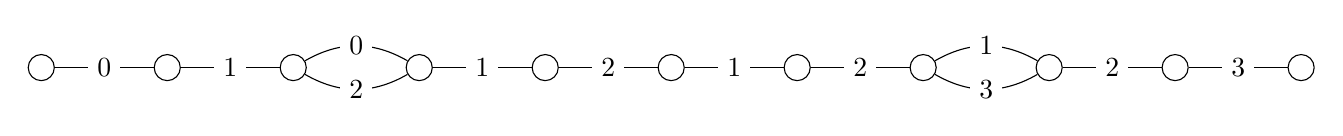
\begin{tikzpicture}[scale=.8]

      \begin{scope}[every node/.style={circle,draw}]
        \node (1)  at (0,0) {};
        \node (2)  at (2,0) {};
        \node (3)  at (4,0) {};
        \node (4)  at (6,0)  {};
        \node (5)  at (8,0)  {};
        \node (6)  at (10,0)  {};
        \node (7)  at (12,0)  {};
        \node (8)  at (14,0)  {};
        \node (9)  at (16,0)  {};
        \node (10) at (18,0)  {};
        \node (11) at (20,0)  {};
      \end{scope}

      \begin{scope}[every node/.style={fill=white}]

        \begin{scope}[every edge/.style={draw}]
          \path (1)  edge node {$0$} (2);
          \path (3)  edge[bend left=30] node {$0$} (4);
          \path (2)  edge node {$1$} (3);
          \path (4)  edge node {$1$} (5);
          \path (6)  edge node {$1$} (7);
          \path (8)  edge[bend left=30] node {$1$} (9);
          \path (3)  edge[bend right=30] node {$2$} (4);
          \path (5)  edge node {$2$} (6);
          \path (7)  edge node {$2$} (8);
          \path (9)  edge node {$2$} (10);
          \path (8)  edge[bend right=30] node {$3$} (9);
          \path (10) edge node {$3$} (11);
        \end{scope}
      \end{scope}

    \end{tikzpicture}
    \caption{[1, 995, 1010, 234]}
  \end{center}
\end{figure}

\begin{figure}[H]
  \begin{center}
    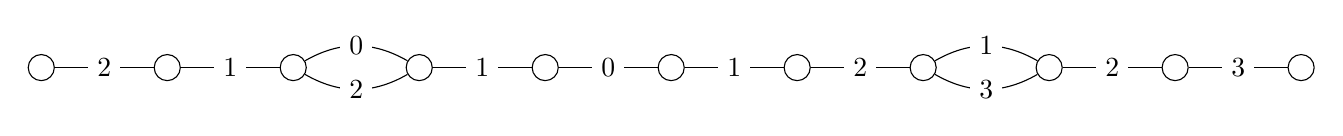
\begin{tikzpicture}[scale=.8]

      \begin{scope}[every node/.style={circle,draw}]
        \node (1)  at (10,0)  {};
        \node (2)  at (8,0)  {};
        \node (3)  at (6,0)  {};
        \node (4)  at (4,0)  {};
        \node (5)  at (2,0) {};
        \node (6)  at (20,0) {};
        \node (7)  at (0,0) {};
        \node (8)  at (18,0)  {};
        \node (9)  at (16,0)  {};
        \node (10) at (14,0) {};
        \node (11) at (12,0) {};
      \end{scope}

      \begin{scope}[every node/.style={fill=white}]

        \begin{scope}[every edge/.style={draw}]
          \path (1)  edge node {$0$} (2);
          \path (3)  edge[bend right=30] node {$0$} (4);
          \path (1)  edge node {$1$} (11);
          \path (2)  edge node {$1$} (3);
          \path (4)  edge node {$1$} (5);
          \path (9)  edge[bend right=30] node {$1$} (10);
          \path (3)  edge[bend left=30] node {$2$} (4);
          \path (5)  edge node {$2$} (7);
          \path (8)  edge node {$2$} (9);
          \path (10) edge node {$2$} (11);
          \path (6)  edge node {$3$} (8);
          \path (9)  edge[bend left=30] node {$3$} (10);
        \end{scope}
      \end{scope}

    \end{tikzpicture}
    \caption{[1, 1075, 1096, 159]}
  \end{center}
\end{figure}

\begin{figure}[H]
  \begin{center}
    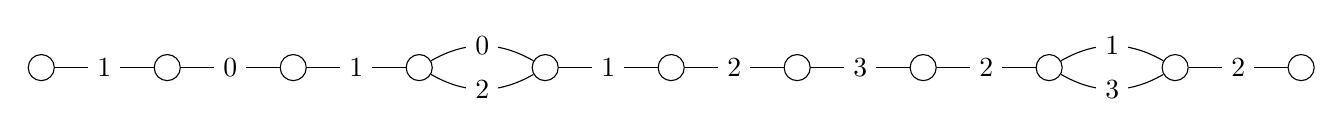
\begin{tikzpicture}[scale=.8]

      \begin{scope}[every node/.style={circle,draw}]
        \node (1)  at (8,0)  {};
        \node (2)  at (6,0)  {};
        \node (3)  at (4,0)  {};
        \node (4)  at (2,0)  {};
        \node (5)  at (0,0)  {};
        \node (6)  at (12,0)  {};
        \node (7)  at (14,0)  {};
        \node (8)  at (20,0) {};
        \node (9)  at (18,0)  {};
        \node (10) at (16,0) {};
        \node (11) at (10,0) {};
      \end{scope}

      \begin{scope}[every node/.style={fill=white}]

        \begin{scope}[every edge/.style={draw}]
          \path (1)  edge[bend right=30] node {$0$} (2);
          \path (3)  edge node {$0$} (4);
          \path (1)  edge node {$1$} (11);
          \path (2)  edge node {$1$} (3);
          \path (4)  edge node {$1$} (5);
          \path (9)  edge[bend right=30] node {$1$} (10);
          \path (1)  edge[bend left=30] node {$2$} (2);
          \path (6)  edge node {$2$} (11);
          \path (7)  edge node {$2$} (10);
          \path (8)  edge node {$2$} (9);
          \path (6)  edge node {$3$} (7);
          \path (9)  edge[bend left=30] node {$3$} (10);
        \end{scope}
      \end{scope}

    \end{tikzpicture}
    \caption{[1, 1075, 5720, 153]}
  \end{center}
\end{figure}

\begin{figure}[H]
  \begin{center}
    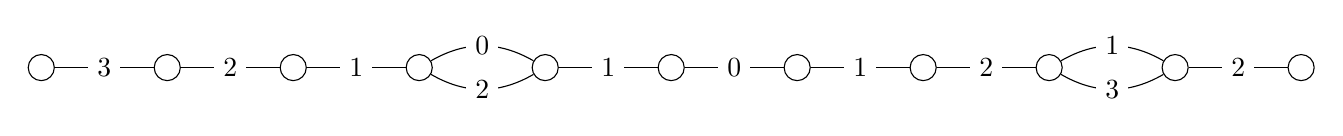
\begin{tikzpicture}[scale=.8]

      \begin{scope}[every node/.style={circle,draw}]
        \node (1)  at (12,0)  {};
        \node (2)  at (10,0)  {};
        \node (3)  at (8,0)  {};
        \node (4)  at (6,0)  {};
        \node (5)  at (4,0) {};
        \node (6)  at (2,0)  {};
        \node (7)  at (0,0)  {};
        \node (8)  at (20,0)  {};
        \node (9)  at (18,0)  {};
        \node (10) at (16,0) {};
        \node (11) at (14,0) {};
      \end{scope}

      \begin{scope}[every node/.style={fill=white}]

        \begin{scope}[every edge/.style={draw}]
          \path (1)  edge node {$0$} (2);
          \path (3)  edge[bend right=30] node {$0$} (4);
          \path (1)  edge node {$1$} (11);
          \path (2)  edge node {$1$} (3);
          \path (4)  edge node {$1$} (5);
          \path (9)  edge[bend right=30] node {$1$} (10);
          \path (3)  edge[bend left=30] node {$2$} (4);
          \path (5)  edge node {$2$} (6);
          \path (8)  edge node {$2$} (9);
          \path (10) edge node {$2$} (11);
          \path (6)  edge node {$3$} (7);
          \path (9)  edge[bend left=30] node {$3$} (10);
        \end{scope}
      \end{scope}

    \end{tikzpicture}
    \caption{[1, 1075, 1088, 153]}
  \end{center}
\end{figure}

\begin{figure}[H]
  \begin{center}
    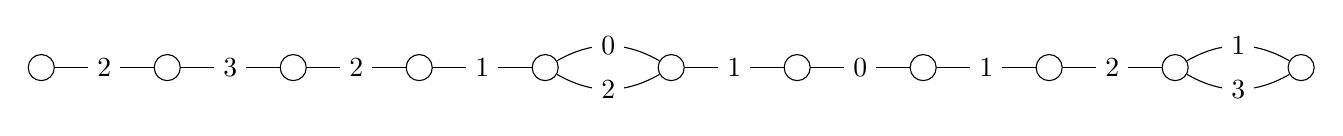
\begin{tikzpicture}[scale=.8]

      \begin{scope}[every node/.style={circle,draw}]
        \node (1)  at (14,0)  {};
        \node (2)  at (12,0)  {};
        \node (3)  at (10,0)  {};
        \node (4)  at (8,0)  {};
        \node (5)  at (6,0) {};
        \node (6)  at (4,0) {};
        \node (7)  at (2,0) {};
        \node (8)  at (0,0)  {};
        \node (9)  at (20,0)  {};
        \node (10) at (18,0) {};
        \node (11) at (16,0) {};
      \end{scope}

      \begin{scope}[every node/.style={fill=white}]

        \begin{scope}[every edge/.style={draw}]
          \path (1)  edge node {$0$} (2);
          \path (3)  edge[bend right=30] node {$0$} (4);
          \path (1)  edge node {$1$} (11);
          \path (2)  edge node {$1$} (3);
          \path (4)  edge node {$1$} (5);
          \path (9)  edge[bend right=30] node {$1$} (10);
          \path (3)  edge[bend left=30] node {$2$} (4);
          \path (5)  edge node {$2$} (6);
          \path (7)  edge node {$2$} (8);
          \path (10) edge node {$2$} (11);
          \path (6)  edge node {$3$} (7);
          \path (9)  edge[bend left=30] node {$3$} (10);
        \end{scope}
      \end{scope}

    \end{tikzpicture}
    \caption{[1, 1075, 1266, 153]}
  \end{center}
\end{figure}

\begin{figure}[H]
  \begin{center}
    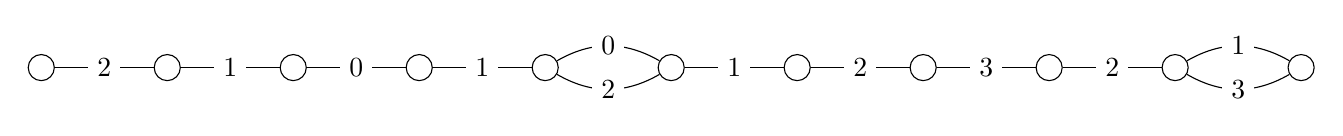
\begin{tikzpicture}[scale=.8]

      \begin{scope}[every node/.style={circle,draw}]
        \node (1)  at (4,0)  {};
        \node (2)  at (6,0)  {};
        \node (3)  at (8,0)  {};
        \node (4)  at (10,0)  {};
        \node (5)  at (12,0) {};
        \node (6)  at (14,0)  {};
        \node (7)  at (0,0) {};
        \node (8)  at (16,0)  {};
        \node (9)  at (20,0)  {};
        \node (10) at (18,0) {};
        \node (11) at (2,0) {};
      \end{scope}

      \begin{scope}[every node/.style={fill=white}]

        \begin{scope}[every edge/.style={draw}]
          \path (1)  edge node {$0$} (2);
          \path (3)  edge[bend left=30] node {$0$} (4);
          \path (1)  edge node {$1$} (11);
          \path (2)  edge node {$1$} (3);
          \path (4)  edge node {$1$} (5);
          \path (9)  edge[bend right=30] node {$1$} (10);
          \path (3)  edge[bend right=30] node {$2$} (4);
          \path (5)  edge node {$2$} (6);
          \path (7)  edge node {$2$} (11);
          \path (8)  edge node {$2$} (10);
          \path (6)  edge node {$3$} (8);
          \path (9)  edge[bend left=30] node {$3$} (10);
        \end{scope}
      \end{scope}

    \end{tikzpicture}
    \caption{[1, 1075, 1579, 159]}
  \end{center}
\end{figure}

\begin{figure}[H]
  \begin{center}
    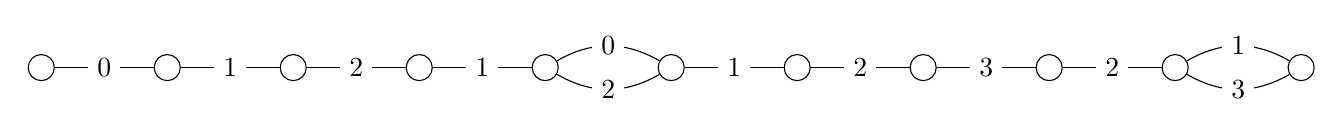
\begin{tikzpicture}[scale=.8]

      \begin{scope}[every node/.style={circle,draw}]
        \node (1)  at (20,0) {};
        \node (2)  at (18,0) {};
        \node (3)  at (16,0) {};
        \node (4)  at (14,0)  {};
        \node (5)  at (12,0)  {};
        \node (6)  at (10,0)  {};
        \node (7)  at (8,0)  {};
        \node (8)  at (6,0)  {};
        \node (9)  at (4,0)  {};
        \node (10) at (2,0)  {};
        \node (11) at (0,0)  {};
      \end{scope}

      \begin{scope}[every node/.style={fill=white}]

        \begin{scope}[every edge/.style={draw}]
          \path (1)  edge[bend left=30] node {$3$} (2);
          \path (3)  edge node {$3$} (4);
          \path (2)  edge node {$2$} (3);
          \path (4)  edge node {$2$} (5);
          \path (6)  edge[bend left=30] node {$2$} (7);
          \path (8)  edge node {$2$} (9);
          \path (1)  edge[bend right=30] node {$1$} (2);
          \path (5)  edge node {$1$} (6);
          \path (7)  edge node {$1$} (8);
          \path (9)  edge node {$1$} (10);
          \path (6)  edge[bend right=30] node {$0$} (7);
          \path (10) edge node {$0$} (11);
        \end{scope}
      \end{scope}

    \end{tikzpicture}
    \caption{[1, 995, 994, 219]}
  \end{center}
\end{figure}

\subsubsection{Longueur 2}

\begin{figure}[H]
  \begin{center}
    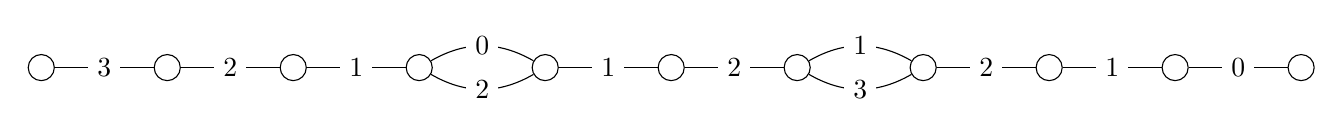
\begin{tikzpicture}[scale=.8]

      \begin{scope}[every node/.style={circle,draw}]
        \node (1)  at (8,0) {};
        \node (2)  at (6,0)  {};
        \node (3)  at (18,0)  {};
        \node (4)  at (20,0)  {};
        \node (5)  at (0,0)  {};
        \node (6)  at (2,0)  {};
        \node (7)  at (4,0)  {};
        \node (8)  at (10,0)  {};
        \node (9)  at (12,0)  {};
        \node (10) at (14,0)  {};
        \node (11) at (16,0) {};
      \end{scope}

      \begin{scope}[every node/.style={fill=white}]

        \begin{scope}[every edge/.style={draw}]
          \path (1)  edge[bend right=30] node {$0$} (2);
          \path (3)  edge node {$0$} (4);
          \path (1)  edge node {$1$} (8);
          \path (2)  edge node {$1$} (7);
          \path (3)  edge node {$1$} (11);
          \path (9)  edge[bend left=30] node {$1$} (10);
          \path (1)  edge[bend left=30] node {$2$} (2);
          \path (6)  edge node {$2$} (7);
          \path (8)  edge node {$2$} (9);
          \path (10) edge node {$2$} (11);
          \path (5)  edge node {$3$} (6);
          \path (9)  edge[bend right=30] node {$3$} (10);
        \end{scope}
      \end{scope}

    \end{tikzpicture}
    \caption{[1, 1029, 998, 147]}
  \end{center}
\end{figure}

\begin{figure}[H]
  \begin{center}
    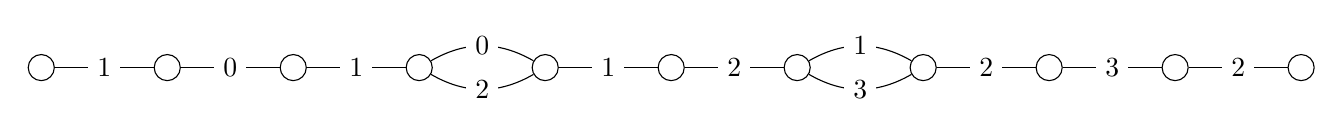
\begin{tikzpicture}[scale=.8]

      \begin{scope}[every node/.style={circle,draw}]
        \node (1)  at (8,0)  {};
        \node (2)  at (6,0)  {};
        \node (3)  at (4,0)  {};
        \node (4)  at (2,0)  {};
        \node (5)  at (0,0) {};
        \node (6)  at (18,0)  {};
        \node (7)  at (20,0)  {};
        \node (8)  at (16,0)  {};
        \node (9)  at (14,0)  {};
        \node (10) at (12,0) {};
        \node (11) at (10,0) {};
      \end{scope}

      \begin{scope}[every node/.style={fill=white}]

        \begin{scope}[every edge/.style={draw}]
          \path (1)  edge[bend right=30] node {$0$} (2);
          \path (3)  edge node {$0$} (4);
          \path (1)  edge node {$1$} (11);
          \path (2)  edge node {$1$} (3);
          \path (4)  edge node {$1$} (5);
          \path (9)  edge[bend right=30] node {$1$} (10);
          \path (1)  edge[bend left=30] node {$2$} (2);
          \path (6)  edge node {$2$} (7);
          \path (8)  edge node {$2$} (9);
          \path (10) edge node {$2$} (11);
          \path (6)  edge node {$3$} (8);
          \path (9)  edge[bend left=30] node {$3$} (10);
        \end{scope}
      \end{scope}

    \end{tikzpicture}
    \caption{[1, 1075, 998, 159]}
  \end{center}
\end{figure}

\begin{figure}[H]
  \begin{center}
    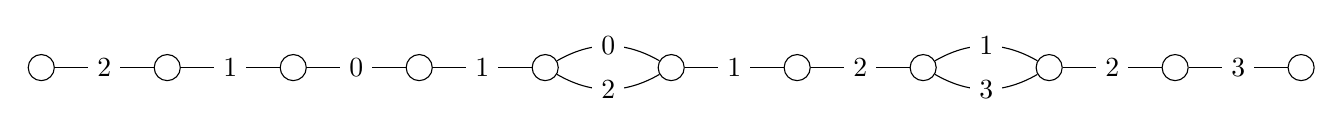
\begin{tikzpicture}[scale=.8]

      \begin{scope}[every node/.style={circle,draw}]
        \node (1)  at (10,0)  {};
        \node (2)  at (8,0)  {};
        \node (3)  at (6,0)  {};
        \node (4)  at (4,0)  {};
        \node (5)  at (2,0) {};
        \node (6)  at (0,0) {};
        \node (7)  at (20,0) {};
        \node (8)  at (18,0)  {};
        \node (9)  at (16,0)  {};
        \node (10) at (14,0) {};
        \node (11) at (12,0) {};
      \end{scope}

      \begin{scope}[every node/.style={fill=white}]

        \begin{scope}[every edge/.style={draw}]
          \path (1)  edge[bend right=30] node {$0$} (2);
          \path (3)  edge node {$0$} (4);
          \path (1)  edge node {$1$} (11);
          \path (2)  edge node {$1$} (3);
          \path (4)  edge node {$1$} (5);
          \path (9)  edge[bend right=30] node {$1$} (10);
          \path (1)  edge[bend left=30] node {$2$} (2);
          \path (5)  edge node {$2$} (6);
          \path (8)  edge node {$2$} (9);
          \path (10) edge node {$2$} (11);
          \path (7)  edge node {$3$} (8);
          \path (9)  edge[bend left=30] node {$3$} (10);
        \end{scope}
      \end{scope}

    \end{tikzpicture}
    \caption{[1, 1075, 1271, 160]}
  \end{center}
\end{figure}

\begin{figure}[H]
  \begin{center}
    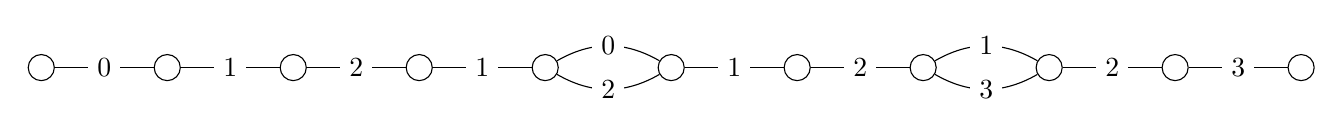
\begin{tikzpicture}[scale=.8]

      \begin{scope}[every node/.style={circle,draw}]
        \node (1)  at (20,0) {};
        \node (2)  at (18,0) {};
        \node (3)  at (16,0) {};
        \node (4)  at (14,0)  {};
        \node (5)  at (12,0)  {};
        \node (6)  at (10,0)  {};
        \node (7)  at (8,0)  {};
        \node (8)  at (6,0)  {};
        \node (9)  at (4,0)  {};
        \node (10) at (2,0)  {};
        \node (11) at (0,0)  {};
      \end{scope}

      \begin{scope}[every node/.style={fill=white}]

        \begin{scope}[every edge/.style={draw}]
          \path (1)  edge node {$3$} (2);
          \path (3)  edge[bend left=30] node {$3$} (4);
          \path (2)  edge node {$2$} (3);
          \path (4)  edge node {$2$} (5);
          \path (6)  edge[bend left=30] node {$2$} (7);
          \path (8)  edge node {$2$} (9);
          \path (3)  edge[bend right=30] node {$1$} (4);
          \path (5)  edge node {$1$} (6);
          \path (7)  edge node {$1$} (8);
          \path (9)  edge node {$1$} (10);
          \path (6)  edge[bend right=30] node {$0$} (7);
          \path (10) edge node {$0$} (11);
        \end{scope}
      \end{scope}

    \end{tikzpicture}
    \caption{[1, 995, 1010, 219]}
  \end{center}
\end{figure}

\begin{figure}[H]
  \begin{center}
    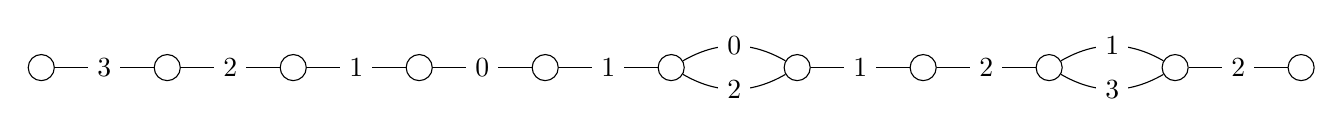
\begin{tikzpicture}[scale=.8]

      \begin{scope}[every node/.style={circle,draw}]
        \node (1)  at (12,0)  {};
        \node (2)  at (10,0)  {};
        \node (3)  at (8,0)  {};
        \node (4)  at (6,0)  {};
        \node (5)  at (4,0) {};
        \node (6)  at (2,0) {};
        \node (7)  at (0,0) {};
        \node (8)  at (20,0)  {};
        \node (9)  at (18,0)  {};
        \node (10) at (16,0) {};
        \node (11) at (14,0) {};
      \end{scope}

      \begin{scope}[every node/.style={fill=white}]

        \begin{scope}[every edge/.style={draw}]
          \path (1)  edge[bend right=30] node {$0$} (2);
          \path (3)  edge node {$0$} (4);
          \path (1)  edge node {$1$} (11);
          \path (2)  edge node {$1$} (3);
          \path (4)  edge node {$1$} (5);
          \path (9)  edge[bend right=30] node {$1$} (10);
          \path (1)  edge[bend left=30] node {$2$} (2);
          \path (5)  edge node {$2$} (6);
          \path (8)  edge node {$2$} (9);
          \path (10) edge node {$2$} (11);
          \path (6)  edge node {$3$} (7);
          \path (9)  edge[bend left=30] node {$3$} (10);
        \end{scope}
      \end{scope}

    \end{tikzpicture}
    \caption{[1, 1075, 1271, 153]}
  \end{center}
\end{figure}

\begin{figure}[H]
  \begin{center}
    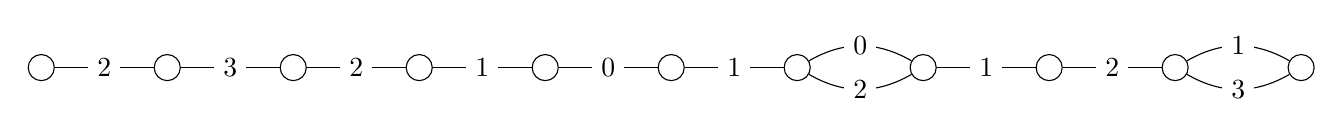
\begin{tikzpicture}[scale=.8]

      \begin{scope}[every node/.style={circle,draw}]
        \node (1)  at (14,0)  {};
        \node (2)  at (12,0)  {};
        \node (3)  at (10,0)  {};
        \node (4)  at (8,0)  {};
        \node (5)  at (6,0) {};
        \node (6)  at (4,0)  {};
        \node (7)  at (2,0) {};
        \node (8)  at (0,0)  {};
        \node (9)  at (20,0)  {};
        \node (10) at (18,0) {};
        \node (11) at (16,0) {};
      \end{scope}

      \begin{scope}[every node/.style={fill=white}]

        \begin{scope}[every edge/.style={draw}]
          \path (1)  edge[bend right=30] node {$0$} (2);
          \path (3)  edge node {$0$} (4);
          \path (1)  edge node {$1$} (11);
          \path (2)  edge node {$1$} (3);
          \path (4)  edge node {$1$} (5);
          \path (9)  edge[bend right=30] node {$1$} (10);
          \path (1)  edge[bend left=30] node {$2$} (2);
          \path (5)  edge node {$2$} (6);
          \path (7)  edge node {$2$} (8);
          \path (10) edge node {$2$} (11);
          \path (6)  edge node {$3$} (7);
          \path (9)  edge[bend left=30] node {$3$} (10);
        \end{scope}
      \end{scope}

    \end{tikzpicture}
    \caption{[1, 1075, 1808, 153]}
  \end{center}
\end{figure}

\begin{figure}[H]
  \begin{center}
    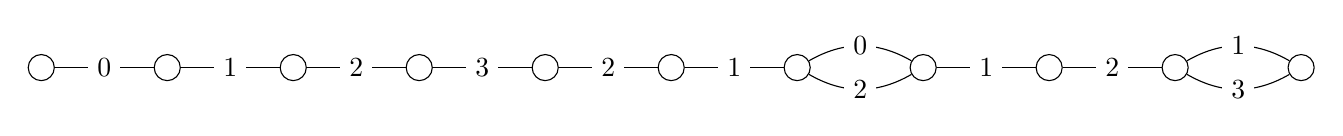
\begin{tikzpicture}[scale=.8]

      \begin{scope}[every node/.style={circle,draw}]
        \node (1)  at (8,0) {};
        \node (2)  at (6,0)  {};
        \node (3)  at (18,0)  {};
        \node (4)  at (20,0)  {};
        \node (5)  at (0,0)  {};
        \node (6)  at (2,0)  {};
        \node (7)  at (4,0)  {};
        \node (8)  at (10,0)  {};
        \node (9)  at (12,0)  {};
        \node (10) at (14,0)  {};
        \node (11) at (16,0) {};
      \end{scope}

      \begin{scope}[every node/.style={fill=white}]

        \begin{scope}[every edge/.style={draw}]
          \path (1)  edge node {$3$} (2);
          \path (3)  edge[bend right=30] node {$3$} (4);
          \path (1)  edge node {$2$} (8);
          \path (2)  edge node {$2$} (7);
          \path (3)  edge node {$2$} (11);
          \path (9)  edge[bend right=30] node {$2$} (10);
          \path (3)  edge[bend left=30] node {$1$} (4);
          \path (6)  edge node {$1$} (7);
          \path (8)  edge node {$1$} (9);
          \path (10) edge node {$1$} (11);
          \path (5)  edge node {$0$} (6);
          \path (9)  edge[bend left=30] node {$0$} (10);
        \end{scope}
      \end{scope}

    \end{tikzpicture}
    \caption{[1, 1029, 1023, 147]}
  \end{center}
\end{figure}

\subsection{Un carré}

\subsubsection{Longueur 4}

\begin{figure}[H]
  \begin{center}
    \begin{tikzpicture}[scale=.8]

      \begin{scope}[every node/.style={circle,draw}]
        \node (1)  at (0,2) {};
        \node (2)  at (2,2) {};
        \node (3)  at (4,2) {};
        \node (4)  at (6,2)  {};
        \node (5)  at (8,2)  {};
        \node (6)  at (10,2)  {};
        \node (7)  at (12,2)  {};
        \node (8)  at (10,0)  {};
        \node (9)  at (12,0)  {};
        \node (10) at (14,0)  {};
        \node (11) at (14,2)  {};
      \end{scope}

      \begin{scope}[every node/.style={fill=white}]

        \begin{scope}[every edge/.style={draw}]
          \path (1)  edge[bend left=30] node {$0$} (2);
          \path (3)  edge node {$0$} (4);
          \path (2)  edge node {$1$} (3);
          \path (4)  edge node {$1$} (5);
          \path (6)  edge node {$1$} (7);
          \path (8)  edge node {$1$} (9);
          \path (1)  edge[bend right=30] node {$2$} (2);
          \path (5)  edge node {$2$} (6);
          \path (7)  edge node {$2$} (11);
          \path (9)  edge node {$2$} (10);
          \path (6)  edge node {$3$} (8);
          \path (7)  edge node {$3$} (9);
        \end{scope}
      \end{scope}

    \end{tikzpicture}
    \caption{[1, 995, 2773, 286]}
  \end{center}
\end{figure}

\begin{figure}[H]
  \begin{center}
    \begin{tikzpicture}[scale=.8]

      \begin{scope}[every node/.style={circle,draw}]
        \node (1)  at (0,2) {};
        \node (2)  at (2,2) {};
        \node (3)  at (4,2) {};
        \node (4)  at (6,2)  {};
        \node (5)  at (8,2)  {};
        \node (6)  at (10,2)  {};
        \node (7)  at (12,2)  {};
        \node (8)  at (12,0)  {};
        \node (9)  at (10,0)  {};
        \node (10) at (8,0)  {};
        \node (11) at (14,0)  {};
      \end{scope}

      \begin{scope}[every node/.style={fill=white}]

        \begin{scope}[every edge/.style={draw}]
          \path (1)  edge[bend left=30] node {$0$} (2);
          \path (3)  edge node {$0$} (4);
          \path (2)  edge node {$1$} (3);
          \path (4)  edge node {$1$} (5);
          \path (6)  edge node {$1$} (7);
          \path (8)  edge node {$1$} (9);
          \path (1)  edge[bend right=30] node {$2$} (2);
          \path (5)  edge node {$2$} (6);
          \path (8)  edge node {$2$} (11);
          \path (9)  edge node {$2$} (10);
          \path (6)  edge node {$3$} (9);
          \path (7)  edge node {$3$} (8);
        \end{scope}
      \end{scope}

    \end{tikzpicture}
    \caption{[1, 995, 2797, 185]}
  \end{center}
\end{figure}

\begin{figure}[H]
  \begin{center}
    \begin{tikzpicture}[scale=.8]

      \begin{scope}[every node/.style={circle,draw}]
        \node (1)  at (0,2) {};
        \node (2)  at (2,2) {};
        \node (3)  at (4,2) {};
        \node (4)  at (6,2)  {};
        \node (5)  at (8,2)  {};
        \node (6)  at (10,2)  {};
        \node (7)  at (12,2)  {};
        \node (8)  at (10,0)  {};
        \node (9)  at (12,0)  {};
        \node (10) at (8,0)  {};
        \node (11) at (14,2)  {};
      \end{scope}

      \begin{scope}[every node/.style={fill=white}]

        \begin{scope}[every edge/.style={draw}]
          \path (1)  edge[bend left=30] node {$0$} (2);
          \path (3)  edge node {$0$} (4);
          \path (2)  edge node {$1$} (3);
          \path (4)  edge node {$1$} (5);
          \path (6)  edge node {$1$} (7);
          \path (8)  edge node {$1$} (9);
          \path (1)  edge[bend right=30] node {$2$} (2);
          \path (5)  edge node {$2$} (6);
          \path (7)  edge node {$2$} (11);
          \path (8)  edge node {$2$} (10);
          \path (6)  edge node {$3$} (8);
          \path (7)  edge node {$3$} (9);
        \end{scope}
      \end{scope}

    \end{tikzpicture}
    \caption{[1, 995, 2703, 286]}
  \end{center}
\end{figure}

\subsubsection{Longueur 2}

\begin{figure}[H]
  \begin{center}
    \begin{tikzpicture}[scale=.8]

      \begin{scope}[every node/.style={circle,draw}]
        \node (1)  at (0,2) {};
        \node (2)  at (2,2) {};
        \node (3)  at (4,2) {};
        \node (4)  at (6,2)  {};
        \node (5)  at (8,2)  {};
        \node (6)  at (10,2)  {};
        \node (7)  at (12,2)  {};
        \node (8)  at (10,0)  {};
        \node (9)  at (12,0)  {};
        \node (10) at (14,0)  {};
        \node (11) at (14,2)  {};
      \end{scope}

      \begin{scope}[every node/.style={fill=white}]

        \begin{scope}[every edge/.style={draw}]
          \path (1)  edge node {$0$} (2);
          \path (3)  edge[bend left=30] node {$0$} (4);
          \path (2)  edge node {$1$} (3);
          \path (4)  edge node {$1$} (5);
          \path (6)  edge node {$1$} (7);
          \path (8)  edge node {$1$} (9);
          \path (3)  edge[bend right=30] node {$2$} (4);
          \path (5)  edge node {$2$} (6);
          \path (7)  edge node {$2$} (11);
          \path (9)  edge node {$2$} (10);
          \path (6)  edge node {$3$} (8);
          \path (7)  edge node {$3$} (9);
        \end{scope}
      \end{scope}

    \end{tikzpicture}
    \caption{[1, 995, 1608, 286]}
  \end{center}
\end{figure}

\begin{figure}[H]
  \begin{center}
    \begin{tikzpicture}[scale=.8]

      \begin{scope}[every node/.style={circle,draw}]
        \node (1)  at (0,2)  {};
        \node (2)  at (2,2)  {};
        \node (3)  at (4,2)  {};
        \node (4)  at (6,2)  {};
        \node (5)  at (8,2) {};
        \node (6)  at (10,2)  {};
        \node (7)  at (12,2) {};
        \node (8)  at (12,0)  {};
        \node (9)  at (10,0)  {};
        \node (10) at (8,0) {};
        \node (11) at (14,0) {};
      \end{scope}

      \begin{scope}[every node/.style={fill=white}]

        \begin{scope}[every edge/.style={draw}]
          \path (1)  edge node {$0$} (2);
          \path (3)  edge[bend left=30] node {$0$} (4);
          \path (2)  edge node {$1$} (3);
          \path (4)  edge node {$1$} (5);
          \path (6)  edge node {$1$} (7);
          \path (8)  edge node {$1$} (9);
          \path (3)  edge[bend right=30] node {$2$} (4);
          \path (5)  edge node {$2$} (6);
          \path (8)  edge node {$2$} (11);
          \path (9)  edge node {$2$} (10);
          \path (6)  edge node {$3$} (9);
          \path (7)  edge node {$3$} (8);
        \end{scope}
      \end{scope}

    \end{tikzpicture}
    \caption{[1, 995, 1618, 185]}
  \end{center}
\end{figure}

\begin{figure}[H]
  \begin{center}
    \begin{tikzpicture}[scale=.8]

      \begin{scope}[every node/.style={circle,draw}]
        \node (1)  at (0,2) {};
        \node (2)  at (2,2) {};
        \node (3)  at (4,2) {};
        \node (4)  at (6,2)  {};
        \node (5)  at (8,2)  {};
        \node (6)  at (10,2)  {};
        \node (7)  at (12,2)  {};
        \node (8)  at (10,0)  {};
        \node (9)  at (12,0)  {};
        \node (10) at (8,0)  {};
        \node (11) at (14,2)  {};
      \end{scope}

      \begin{scope}[every node/.style={fill=white}]

        \begin{scope}[every edge/.style={draw}]
          \path (1)  edge node {$0$} (2);
          \path (3)  edge[bend left=30] node {$0$} (4);
          \path (2)  edge node {$1$} (3);
          \path (4)  edge node {$1$} (5);
          \path (6)  edge node {$1$} (7);
          \path (8)  edge node {$1$} (9);
          \path (3)  edge[bend right=30] node {$2$} (4);
          \path (5)  edge node {$2$} (6);
          \path (7)  edge node {$2$} (11);
          \path (8)  edge node {$2$} (10);
          \path (6)  edge node {$3$} (8);
          \path (7)  edge node {$3$} (9);
        \end{scope}
      \end{scope}

    \end{tikzpicture}
    \caption{[1, 995, 1579, 286]}
  \end{center}
\end{figure}

\begin{figure}[H]
  \begin{center}
    \begin{tikzpicture}[scale=.8]

      \begin{scope}[every node/.style={circle,draw}]
        \node (1)  at (14,2) {};
        \node (2)  at (12,2)  {};
        \node (3)  at (2,2)  {};
        \node (4)  at (0,2)  {};
        \node (5)  at (4,2)  {};
        \node (6)  at (10,2)  {};
        \node (7)  at (8,0)  {};
        \node (8)  at (8,2)  {};
        \node (9)  at (6,2)  {};
        \node (10) at (6,0)  {};
        \node (11) at (4,0) {};
      \end{scope}

      \begin{scope}[every node/.style={fill=white}]

        \begin{scope}[every edge/.style={draw}]
          \path (1)  edge node {$0$} (2);
          \path (3)  edge[bend right=30] node {$0$} (4);
          \path (2)  edge node {$1$} (6);
          \path (3)  edge node {$1$} (5);
          \path (7)  edge node {$1$} (8);
          \path (9)  edge node {$1$} (10);
          \path (3)  edge[bend left=30] node {$2$} (4);
          \path (5)  edge node {$2$} (9);
          \path (6)  edge node {$2$} (8);
          \path (10) edge node {$2$} (11);
          \path (7)  edge node {$3$} (10);
          \path (8)  edge node {$3$} (9);
        \end{scope}
      \end{scope}

    \end{tikzpicture}
    \caption{[1, 1013, 1195, 267]}
  \end{center}
\end{figure}

\begin{figure}[H]
  \begin{center}
    \begin{tikzpicture}[scale=.8]

      \begin{scope}[every node/.style={circle,draw}]
        \node (1)  at (14,2) {};
        \node (2)  at (12,2)  {};
        \node (3)  at (2,2)  {};
        \node (4)  at (0,2)  {};
        \node (5)  at (4,2)  {};
        \node (6)  at (10,2)  {};
        \node (7)  at (6,0)  {};
        \node (8)  at (6,2)  {};
        \node (9)  at (8,2)  {};
        \node (10) at (8,0)  {};
        \node (11) at (10,0) {};
      \end{scope}

      \begin{scope}[every node/.style={fill=white}]

        \begin{scope}[every edge/.style={draw}]
          \path (1)  edge node {$0$} (2);
          \path (3)  edge[bend right=30] node {$0$} (4);
          \path (2)  edge node {$1$} (6);
          \path (3)  edge node {$1$} (5);
          \path (7)  edge node {$1$} (8);
          \path (9)  edge node {$1$} (10);
          \path (3)  edge[bend left=30] node {$2$} (4);
          \path (5)  edge node {$2$} (8);
          \path (6)  edge node {$2$} (9);
          \path (10) edge node {$2$} (11);
          \path (7)  edge node {$3$} (10);
          \path (8)  edge node {$3$} (9);
        \end{scope}
      \end{scope}

    \end{tikzpicture}
    \caption{[1, 1013, 1381, 267]}
  \end{center}
\end{figure}

\begin{figure}[H]
  \begin{center}
    \begin{tikzpicture}[scale=.8]

      \begin{scope}[every node/.style={circle,draw}]
        \node (1)  at (14,0) {};
        \node (2)  at (12,0)  {};
        \node (3)  at (2,2)  {};
        \node (4)  at (0,2)  {};
        \node (5)  at (4,2)  {};
        \node (6)  at (10,0)  {};
        \node (7)  at (6,0)  {};
        \node (8)  at (8,0)  {};
        \node (9)  at (6,2)  {};
        \node (10) at (8,2)  {};
        \node (11) at (10,2) {};
      \end{scope}

      \begin{scope}[every node/.style={fill=white}]

        \begin{scope}[every edge/.style={draw}]
          \path (1)  edge node {$0$} (2);
          \path (3)  edge[bend right=30] node {$0$} (4);
          \path (2)  edge node {$1$} (6);
          \path (3)  edge node {$1$} (5);
          \path (7)  edge node {$1$} (8);
          \path (9)  edge node {$1$} (10);
          \path (3)  edge[bend left=30] node {$2$} (4);
          \path (5)  edge node {$2$} (9);
          \path (6)  edge node {$2$} (8);
          \path (10) edge node {$2$} (11);
          \path (7)  edge node {$3$} (9);
          \path (8)  edge node {$3$} (10);
        \end{scope}
      \end{scope}

    \end{tikzpicture}
    \caption{[1, 1013, 1195, 381]}
  \end{center}
\end{figure}

\begin{figure}[H]
  \begin{center}
    \begin{tikzpicture}[scale=.8]

      \begin{scope}[every node/.style={circle,draw}]
        \node (1)  at (14,0) {};
        \node (2)  at (12,0)  {};
        \node (3)  at (2,2)  {};
        \node (4)  at (0,2)  {};
        \node (5)  at (4,2)  {};
        \node (6)  at (10,0)  {};
        \node (7)  at (8,2)  {};
        \node (8)  at (6,2)  {};
        \node (9)  at (8,0)  {};
        \node (10) at (6,0)  {};
        \node (11) at (4,0) {};
      \end{scope}

      \begin{scope}[every node/.style={fill=white}]

        \begin{scope}[every edge/.style={draw}]
          \path (1)  edge node {$0$} (2);
          \path (3)  edge[bend right=30] node {$0$} (4);
          \path (2)  edge node {$1$} (6);
          \path (3)  edge node {$1$} (5);
          \path (7)  edge node {$1$} (8);
          \path (9)  edge node {$1$} (10);
          \path (3)  edge[bend left=30] node {$2$} (4);
          \path (5)  edge node {$2$} (8);
          \path (6)  edge node {$2$} (9);
          \path (10) edge node {$2$} (11);
          \path (7)  edge node {$3$} (9);
          \path (8)  edge node {$3$} (10);
        \end{scope}
      \end{scope}

    \end{tikzpicture}
    \caption{[1, 1013, 1381, 381] d}
  \end{center}
\end{figure}

\begin{figure}[H]
  \begin{center}
    \begin{tikzpicture}[scale=.8]

      \begin{scope}[every node/.style={circle,draw}]
        \node (1)  at (12,2) {};
        \node (2)  at (10,2)  {};
        \node (3)  at (0,2)  {};
        \node (4)  at (-2,2)  {};
        \node (5)  at (2,2)  {};
        \node (6)  at (8,2)  {};
        \node (7)  at (6,2)  {};
        \node (8)  at (4,2)  {};
        \node (9)  at (4,0)  {};
        \node (10) at (6,0)  {};
        \node (11) at (2,0) {};
      \end{scope}

      \begin{scope}[every node/.style={fill=white}]

        \begin{scope}[every edge/.style={draw}]
          \path (1)  edge node {$0$} (2);
          \path (3)  edge[bend right=30] node {$0$} (4);
          \path (2)  edge node {$1$} (6);
          \path (3)  edge node {$1$} (5);
          \path (7)  edge node {$1$} (8);
          \path (9)  edge node {$1$} (10);
          \path (3)  edge[bend left=30] node {$2$} (4);
          \path (5)  edge node {$2$} (8);
          \path (6)  edge node {$2$} (7);
          \path (9)  edge node {$2$} (11);
          \path (7)  edge node {$3$} (10);
          \path (8)  edge node {$3$} (9);
        \end{scope}
      \end{scope}

    \end{tikzpicture}
    \caption{[1, 1013, 6336, 267]}
  \end{center}
\end{figure}

\begin{figure}[H]
  \begin{center}
    \begin{tikzpicture}[scale=.8]

      \begin{scope}[every node/.style={circle,draw}]
        \node (1)  at (12,2) {};
        \node (2)  at (10,2)  {};
        \node (3)  at (0,2)  {};
        \node (4)  at (-2,2)  {};
        \node (5)  at (2,2)  {};
        \node (6)  at (8,2)  {};
        \node (7)  at (6,2)  {};
        \node (8)  at (4,2)  {};
        \node (9)  at (6,0)  {};
        \node (10) at (4,0)  {};
        \node (11) at (8,0) {};
      \end{scope}

      \begin{scope}[every node/.style={fill=white}]

        \begin{scope}[every edge/.style={draw}]
          \path (1)  edge node {$0$} (2);
          \path (3)  edge[bend right=30] node {$0$} (4);
          \path (2)  edge node {$1$} (6);
          \path (3)  edge node {$1$} (5);
          \path (7)  edge node {$1$} (8);
          \path (9)  edge node {$1$} (10);
          \path (3)  edge[bend left=30] node {$2$} (4);
          \path (5)  edge node {$2$} (8);
          \path (6)  edge node {$2$} (7);
          \path (9)  edge node {$2$} (11);
          \path (7)  edge node {$3$} (9);
          \path (8)  edge node {$3$} (10);
        \end{scope}
      \end{scope}

    \end{tikzpicture}
    \caption{[1, 1013, 6336, 381]}
  \end{center}
\end{figure}

\subsection{Deux carrés}

\subsubsection{Longueur 4}

\begin{figure}[H]
  \begin{center}
    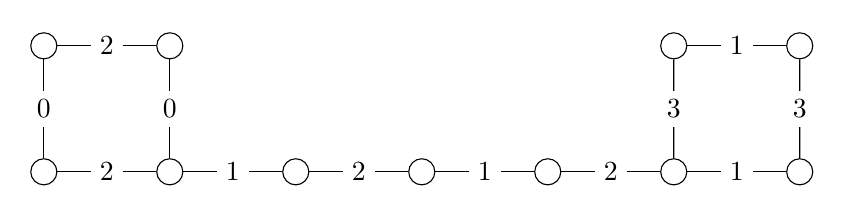
\begin{tikzpicture}[scale=.8]

      \begin{scope}[every node/.style={circle,draw}]
        \node (1)  at (2,2)  {};
        \node (2)  at (2,0)  {};
        \node (3)  at (0,0)  {};
        \node (4)  at (0,2)  {};
        \node (5)  at (4,0)  {};
        \node (6)  at (6,0)  {};
        \node (7)  at (8,0)  {};
        \node (8)  at (10,0)  {};
        \node (9)  at (12,0)  {};
        \node (10) at (12,2) {};
        \node (11) at (10,2) {};
      \end{scope}

      \begin{scope}[every node/.style={fill=white}]

        \begin{scope}[every edge/.style={draw}]
          \path (1)  edge node {$0$} (2);
          \path (3)  edge node {$0$} (4);
          \path (2)  edge node {$1$} (5);
          \path (6)  edge node {$1$} (7);
          \path (8)  edge node {$1$} (9);
          \path (10) edge node {$1$} (11);
          \path (1)  edge node {$2$} (4);
          \path (2)  edge node {$2$} (3);
          \path (5)  edge node {$2$} (6);
          \path (7)  edge node {$2$} (8);
          \path (8)  edge node {$3$} (11);
          \path (9)  edge node {$3$} (10);
        \end{scope}
      \end{scope}

    \end{tikzpicture}
    \caption{[1, 1009, 993, 358]}
  \end{center}
\end{figure}

\subsubsection{Longueur 2}

\begin{figure}[H]
  \begin{center}
    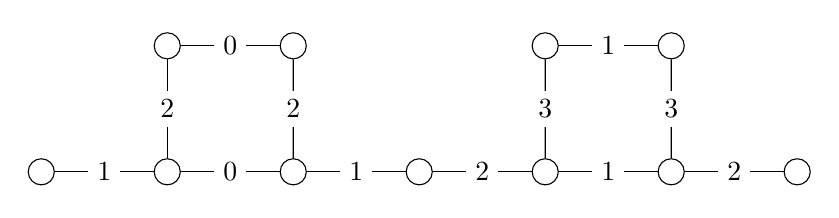
\begin{tikzpicture}[scale=.8]

      \begin{scope}[every node/.style={circle,draw}]
        \node (1)  at (4,0)  {};
        \node (2)  at (2,0)  {};
        \node (3)  at (2,2)  {};
        \node (4)  at (4,2)  {};
        \node (5)  at (0,0)  {};
        \node (6)  at (6,0)  {};
        \node (7)  at (8,2)  {};
        \node (8)  at (10,2) {};
        \node (9)  at (8,0)  {};
        \node (10) at (10,0) {};
        \node (11) at (12,0) {};
      \end{scope}

      \begin{scope}[every node/.style={fill=white}]

        \begin{scope}[every edge/.style={draw}]
          \path (1)  edge node {$0$} (2);
          \path (3)  edge node {$0$} (4);
          \path (1)  edge node {$1$} (6);
          \path (2)  edge node {$1$} (5);
          \path (7)  edge node {$1$} (8);
          \path (9)  edge node {$1$} (10);
          \path (1)  edge node {$2$} (4);
          \path (2)  edge node {$2$} (3);
          \path (6)  edge node {$2$} (9);
          \path (10) edge node {$2$} (11);
          \path (7)  edge node {$3$} (9);
          \path (8)  edge node {$3$} (10);
        \end{scope}
      \end{scope}

    \end{tikzpicture}
    \caption{[1, 1002, 1872, 381] d}
  \end{center}
\end{figure}

\begin{figure}[H]
  \begin{center}
    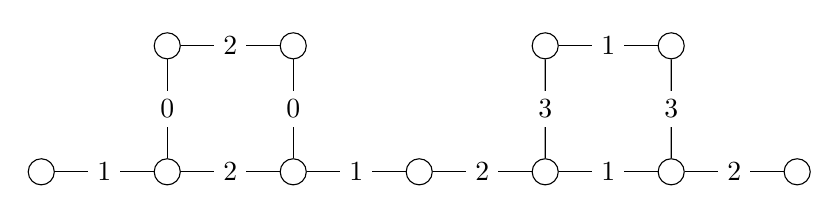
\begin{tikzpicture}[scale=.8]

      \begin{scope}[every node/.style={circle,draw}]
        \node (1)  at (0,2) {};
        \node (2)  at (0,0)  {};
        \node (3)  at (-2,0)  {};
        \node (4)  at (-2,2)  {};
        \node (5)  at (-4,0)  {};
        \node (6)  at (2,0)  {};
        \node (7)  at (6,2)  {};
        \node (8)  at (4,2)  {};
        \node (9)  at (4,0)  {};
        \node (10) at (6,0)  {};
        \node (11) at (8,0) {};
      \end{scope}

      \begin{scope}[every node/.style={fill=white}]

        \begin{scope}[every edge/.style={draw}]
          \path (1)  edge node {$0$} (2);
          \path (3)  edge node {$0$} (4);
          \path (2)  edge node {$1$} (6);
          \path (3)  edge node {$1$} (5);
          \path (7)  edge node {$1$} (8);
          \path (9)  edge node {$1$} (10);
          \path (1)  edge node {$2$} (4);
          \path (2)  edge node {$2$} (3);
          \path (6)  edge node {$2$} (9);
          \path (10) edge node {$2$} (11);
          \path (7)  edge node {$3$} (10);
          \path (8)  edge node {$3$} (9);
        \end{scope}
      \end{scope}

    \end{tikzpicture}
    \caption{[1, 1013, 1872, 267] d}
  \end{center}
\end{figure}

\begin{figure}[H]
  \begin{center}
    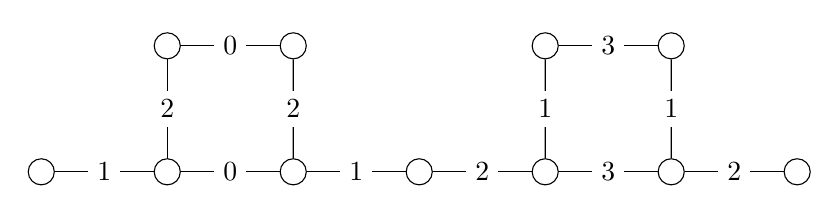
\begin{tikzpicture}[scale=.8]

      \begin{scope}[every node/.style={circle,draw}]
        \node (1)  at (4,0)  {};
        \node (2)  at (2,0)  {};
        \node (3)  at (2,2)  {};
        \node (4)  at (4,2)  {};
        \node (5)  at (0,0)  {};
        \node (6)  at (6,0)  {};
        \node (7)  at (8,0)  {};
        \node (8)  at (8,2) {};
        \node (9)  at (10,2) {};
        \node (10) at (10,0) {};
        \node (11) at (12,0) {};
      \end{scope}

      \begin{scope}[every node/.style={fill=white}]

        \begin{scope}[every edge/.style={draw}]
          \path (1)  edge node {$0$} (2);
          \path (3)  edge node {$0$} (4);
          \path (1)  edge node {$1$} (6);
          \path (2)  edge node {$1$} (5);
          \path (7)  edge node {$1$} (8);
          \path (9)  edge node {$1$} (10);
          \path (1)  edge node {$2$} (4);
          \path (2)  edge node {$2$} (3);
          \path (6)  edge node {$2$} (7);
          \path (10) edge node {$2$} (11);
          \path (7)  edge node {$3$} (10);
          \path (8)  edge node {$3$} (9);
        \end{scope}
      \end{scope}

    \end{tikzpicture}
    \caption{[1, 1002, 1737, 267]}
  \end{center}
\end{figure}

\begin{figure}[H]
  \begin{center}
    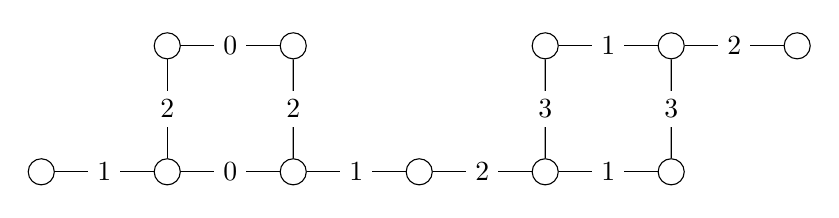
\begin{tikzpicture}[scale=.8]

      \begin{scope}[every node/.style={circle,draw}]
        \node (1)  at (4,0)  {};
        \node (2)  at (2,0)  {};
        \node (3)  at (2,2)  {};
        \node (4)  at (4,2)  {};
        \node (5)  at (0,0)  {};
        \node (6)  at (6,0)  {};
        \node (7)  at (8,0)  {};
        \node (8)  at (10,0) {};
        \node (9)  at (8,2) {};
        \node (10) at (10,2) {};
        \node (11) at (12,2) {};
      \end{scope}

      \begin{scope}[every node/.style={fill=white}]

        \begin{scope}[every edge/.style={draw}]
          \path (1)  edge node {$0$} (2);
          \path (3)  edge node {$0$} (4);
          \path (1)  edge node {$1$} (6);
          \path (2)  edge node {$1$} (5);
          \path (7)  edge node {$1$} (8);
          \path (9)  edge node {$1$} (10);
          \path (1)  edge node {$2$} (4);
          \path (2)  edge node {$2$} (3);
          \path (6)  edge node {$2$} (7);
          \path (10) edge node {$2$} (11);
          \path (7)  edge node {$3$} (9);
          \path (8)  edge node {$3$} (10);
        \end{scope}
      \end{scope}

    \end{tikzpicture}
    \caption{[1, 1002, 1737, 381]}
  \end{center}
\end{figure}

\begin{figure}[H]
  \begin{center}
    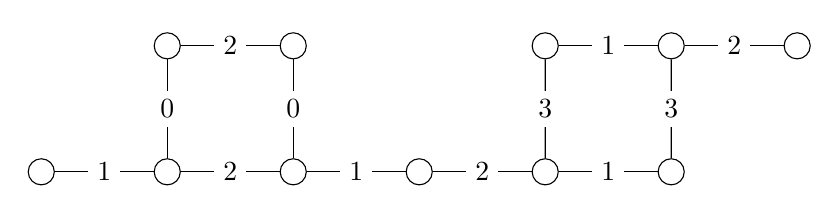
\begin{tikzpicture}[scale=.8]

      \begin{scope}[every node/.style={circle,draw}]
        \node (1)  at (0,2) {};
        \node (2)  at (0,0)  {};
        \node (3)  at (-2,0)  {};
        \node (4)  at (-2,2)  {};
        \node (5)  at (-4,0)  {};
        \node (6)  at (2,0)  {};
        \node (7)  at (4,0)  {};
        \node (8)  at (6,0)  {};
        \node (9)  at (4,2)  {};
        \node (10) at (6,2)  {};
        \node (11) at (8,2) {};
      \end{scope}

      \begin{scope}[every node/.style={fill=white}]

        \begin{scope}[every edge/.style={draw}]
          \path (1)  edge node {$0$} (2);
          \path (3)  edge node {$0$} (4);
          \path (2)  edge node {$1$} (6);
          \path (3)  edge node {$1$} (5);
          \path (7)  edge node {$1$} (8);
          \path (9)  edge node {$1$} (10);
          \path (1)  edge node {$2$} (4);
          \path (2)  edge node {$2$} (3);
          \path (6)  edge node {$2$} (7);
          \path (10) edge node {$2$} (11);
          \path (7)  edge node {$3$} (9);
          \path (8)  edge node {$3$} (10);
        \end{scope}
      \end{scope}

    \end{tikzpicture}
    \caption{[1, 1013, 1737, 381]}
  \end{center}
\end{figure}

\begin{figure}[H]
  \begin{center}
    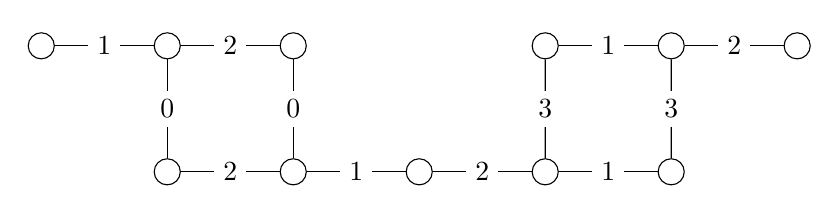
\begin{tikzpicture}[scale=.8]

      \begin{scope}[every node/.style={circle,draw}]
        \node (1)  at (0,2) {};
        \node (2)  at (0,0)  {};
        \node (3)  at (-2,2)  {};
        \node (4)  at (-2,0)  {};
        \node (5)  at (-4,2)  {};
        \node (6)  at (2,0)  {};
        \node (7)  at (4,0)  {};
        \node (8)  at (6,0)  {};
        \node (9)  at (4,2)  {};
        \node (10) at (6,2)  {};
        \node (11) at (8,2) {};
      \end{scope}

      \begin{scope}[every node/.style={fill=white}]

        \begin{scope}[every edge/.style={draw}]
          \path (1)  edge node {$0$} (2);
          \path (3)  edge node {$0$} (4);
          \path (2)  edge node {$1$} (6);
          \path (3)  edge node {$1$} (5);
          \path (7)  edge node {$1$} (8);
          \path (9)  edge node {$1$} (10);
          \path (1)  edge node {$2$} (3);
          \path (2)  edge node {$2$} (4);
          \path (6)  edge node {$2$} (7);
          \path (10) edge node {$2$} (11);
          \path (7)  edge node {$3$} (9);
          \path (8)  edge node {$3$} (10);
        \end{scope}
      \end{scope}

    \end{tikzpicture}
    \caption{[1, 1013, 1738, 381]}
  \end{center}
\end{figure}

\begin{figure}[H]
  \begin{center}
    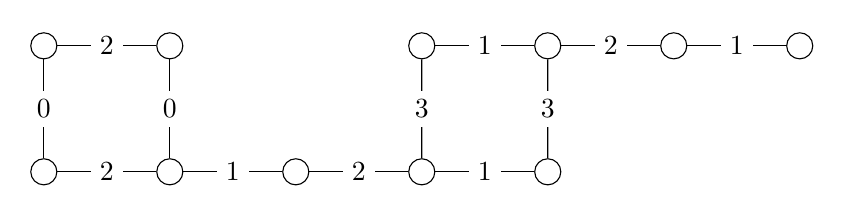
\begin{tikzpicture}[scale=.8]

      \begin{scope}[every node/.style={circle,draw}]
        \node (1)  at (2,2)  {};
        \node (2)  at (2,0)  {};
        \node (3)  at (0,0)  {};
        \node (4)  at (0,2)  {};
        \node (5)  at (4,0)  {};
        \node (6)  at (6,0)  {};
        \node (7)  at (8,0)  {};
        \node (8)  at (8,2)  {};
        \node (9)  at (6,2)  {};
        \node (10) at (10,2)  {};
        \node (11) at (12,2) {};
      \end{scope}

      \begin{scope}[every node/.style={fill=white}]

        \begin{scope}[every edge/.style={draw}]
          \path (1)  edge node {$0$} (2);
          \path (3)  edge node {$0$} (4);
          \path (2)  edge node {$1$} (5);
          \path (6)  edge node {$1$} (7);
          \path (8)  edge node {$1$} (9);
          \path (10) edge node {$1$} (11);
          \path (1)  edge node {$2$} (4);
          \path (2)  edge node {$2$} (3);
          \path (5)  edge node {$2$} (6);
          \path (8)  edge node {$2$} (10);
          \path (6)  edge node {$3$} (9);
          \path (7)  edge node {$3$} (8);
        \end{scope}
      \end{scope}

    \end{tikzpicture}
    \caption{[1, 1009, 3259, 185]}
  \end{center}
\end{figure}

\begin{figure}[H]
  \begin{center}
    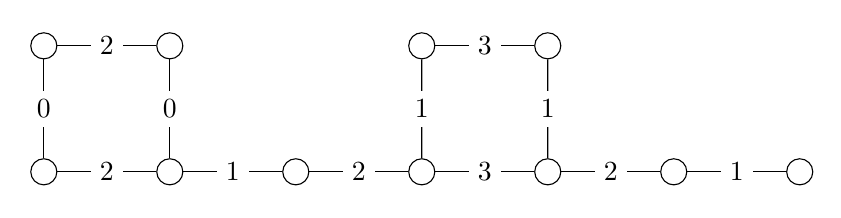
\begin{tikzpicture}[scale=.8]

      \begin{scope}[every node/.style={circle,draw}]
        \node (1)  at (2,2)  {};
        \node (2)  at (2,0)  {};
        \node (3)  at (0,0)  {};
        \node (4)  at (0,2)  {};
        \node (5)  at (4,0)  {};
        \node (6)  at (6,0)  {};
        \node (7)  at (6,2)  {};
        \node (8)  at (8,0)  {};
        \node (9)  at (8,2)  {};
        \node (10) at (10,0)  {};
        \node (11) at (12,0) {};
      \end{scope}

      \begin{scope}[every node/.style={fill=white}]

        \begin{scope}[every edge/.style={draw}]
          \path (1)  edge node {$0$} (2);
          \path (3)  edge node {$0$} (4);
          \path (2)  edge node {$1$} (5);
          \path (6)  edge node {$1$} (7);
          \path (8)  edge node {$1$} (9);
          \path (10) edge node {$1$} (11);
          \path (1)  edge node {$2$} (4);
          \path (2)  edge node {$2$} (3);
          \path (5)  edge node {$2$} (6);
          \path (8)  edge node {$2$} (10);
          \path (6)  edge node {$3$} (8);
          \path (7)  edge node {$3$} (9);
        \end{scope}
      \end{scope}

    \end{tikzpicture}
    \caption{[1, 1009, 3259, 286]}
  \end{center}
\end{figure}

\begin{figure}[H]
  \begin{center}
    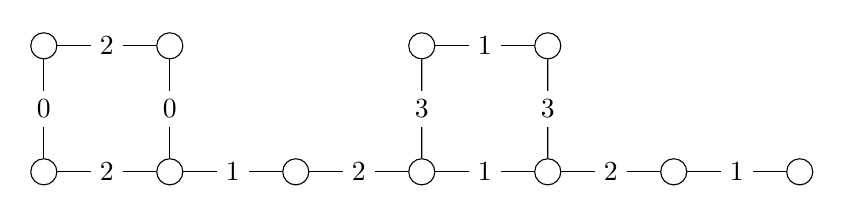
\begin{tikzpicture}[scale=.8]

      \begin{scope}[every node/.style={circle,draw}]
        \node (1)  at (2,2)  {};
        \node (2)  at (2,0)  {};
        \node (3)  at (0,2)  {};
        \node (4)  at (0,0)  {};
        \node (5)  at (4,0)  {};
        \node (6)  at (6,0)  {};
        \node (7)  at (8,0)  {};
        \node (8)  at (10,0)  {};
        \node (9)  at (12,0)  {};
        \node (10) at (8,2) {};
        \node (11) at (6,2) {};
      \end{scope}

      \begin{scope}[every node/.style={fill=white}]

        \begin{scope}[every edge/.style={draw}]
          \path (1)  edge node {$0$} (2);
          \path (3)  edge node {$0$} (4);
          \path (2)  edge node {$1$} (5);
          \path (6)  edge node {$1$} (7);
          \path (8)  edge node {$1$} (9);
          \path (10) edge node {$1$} (11);
          \path (1)  edge node {$2$} (3);
          \path (2)  edge node {$2$} (4);
          \path (5)  edge node {$2$} (6);
          \path (7)  edge node {$2$} (8);
          \path (6)  edge node {$3$} (11);
          \path (7)  edge node {$3$} (10);
        \end{scope}
      \end{scope}

    \end{tikzpicture}
    \caption{[1, 1009, 993, 344]}
  \end{center}
\end{figure}


\section{Trois 4-transpositions}

\subsection{Longueur 1}

\begin{figure}[H]
  \begin{center}
    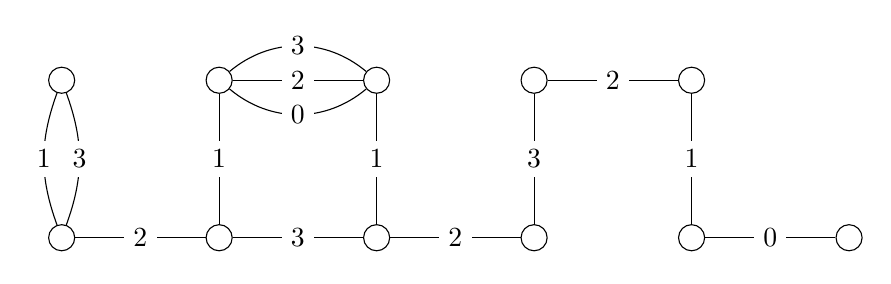
\begin{tikzpicture}

      \begin{scope}[every node/.style={circle,draw}]
        \node (1)  at (2,2)  {};
        \node (2)  at (4,2)  {};
        \node (3)  at (8,0)  {};
        \node (4)  at (10,0) {};
        \node (5)  at (6,0)  {};
        \node (6)  at (6,2)  {};
        \node (7)  at (4,0)  {};
        \node (8)  at (2,0)  {};
        \node (9)  at (0,0)  {};
        \node (10) at (0,2)  {};
        \node (11) at (8,2)  {};
      \end{scope}

      \begin{scope}[every node/.style={fill=white}]

        \begin{scope}[every edge/.style={draw}]
          \path (1)  edge[bend right=40] node {$0$} (2);
          \path (3)  edge node {$0$} (4);
          \path (1)  edge node {$1$} (8);
          \path (2)  edge node {$1$} (7);
          \path (3)  edge node {$1$} (11);
          \path (9)  edge[bend left=20] node {$1$} (10);
          \path (1)  edge node {$2$} (2);
          \path (5)  edge node {$2$} (7);
          \path (6)  edge node {$2$} (11);
          \path (8)  edge node {$2$} (9);
          \path (1)  edge[bend left=40] node {$3$} (2);
          \path (5)  edge node {$3$} (6);
          \path (7)  edge node {$3$} (8);
          \path (9)  edge[bend right=20] node {$3$} (10);
        \end{scope}
      \end{scope}

    \end{tikzpicture}
    \caption{[1, 1029, 8427, 994]}
  \end{center}
\end{figure}

\begin{figure}[H]
  \begin{center}
    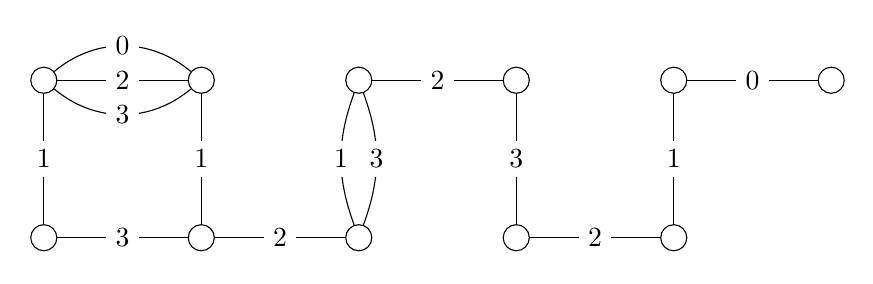
\begin{tikzpicture}

      \begin{scope}[every node/.style={circle,draw}]
        \node (1)  at (2,2)  {};
        \node (2)  at (0,2)  {};
        \node (3)  at (8,2)  {};
        \node (4)  at (10,2) {};
        \node (5)  at (6,2)  {};
        \node (6)  at (6,0)  {};
        \node (7)  at (0,0)  {};
        \node (8)  at (2,0)  {};
        \node (9)  at (4,0)  {};
        \node (10) at (4,2)  {};
        \node (11) at (8,0)  {};
      \end{scope}

      \begin{scope}[every node/.style={fill=white}]

        \begin{scope}[every edge/.style={draw}]
          \path (1)  edge[bend right=40] node {$0$} (2);
          \path (3)  edge node {$0$} (4);
          \path (1)  edge node {$1$} (8);
          \path (2)  edge node {$1$} (7);
          \path (3)  edge node {$1$} (11);
          \path (9)  edge[bend left=20] node {$1$} (10);
          \path (1)  edge node {$2$} (2);
          \path (5)  edge node {$2$} (10);
          \path (6)  edge node {$2$} (11);
          \path (8)  edge node {$2$} (9);
          \path (1)  edge[bend left=40] node {$3$} (2);
          \path (5)  edge node {$3$} (6);
          \path (7)  edge node {$3$} (8);
          \path (9)  edge[bend right=20] node {$3$} (10);
        \end{scope}
      \end{scope}

    \end{tikzpicture}
    \caption{[1, 1029, 8827, 994]}
  \end{center}
\end{figure}

\begin{figure}[H]
  \begin{center}
    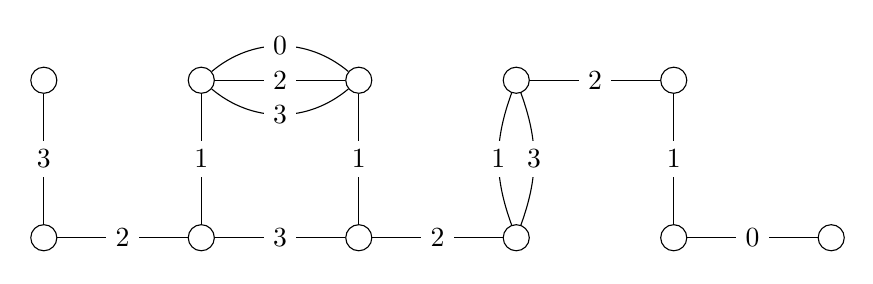
\begin{tikzpicture}

      \begin{scope}[every node/.style={circle,draw}]
        \node (1)  at (4,2)  {};
        \node (2)  at (2,2)  {};
        \node (3)  at (8,0)  {};
        \node (4)  at (10,0) {};
        \node (5)  at (0,2)  {};
        \node (6)  at (0,0)  {};
        \node (7)  at (2,0)  {};
        \node (8)  at (4,0)  {};
        \node (9)  at (6,0)  {};
        \node (10) at (6,2)  {};
        \node (11) at (8,2)  {};
      \end{scope}

      \begin{scope}[every node/.style={fill=white}]

        \begin{scope}[every edge/.style={draw}]
          \path (1)  edge[bend right=40] node {$0$} (2);
          \path (3)  edge node {$0$} (4);
          \path (1)  edge node {$1$} (8);
          \path (2)  edge node {$1$} (7);
          \path (3)  edge node {$1$} (11);
          \path (9)  edge[bend left=20] node {$1$} (10);
          \path (1)  edge node {$2$} (2);
          \path (6)  edge node {$2$} (7);
          \path (8)  edge node {$2$} (9);
          \path (10) edge node {$2$} (11);
          \path (1)  edge[bend left=40] node {$3$} (2);
          \path (5)  edge node {$3$} (6);
          \path (7)  edge node {$3$} (8);
          \path (9)  edge[bend right=20] node {$3$} (10);
        \end{scope}
      \end{scope}

    \end{tikzpicture}
    \caption{[1, 1029, 998, 994]}
  \end{center}
\end{figure}

\begin{figure}[H]
  \begin{center}
    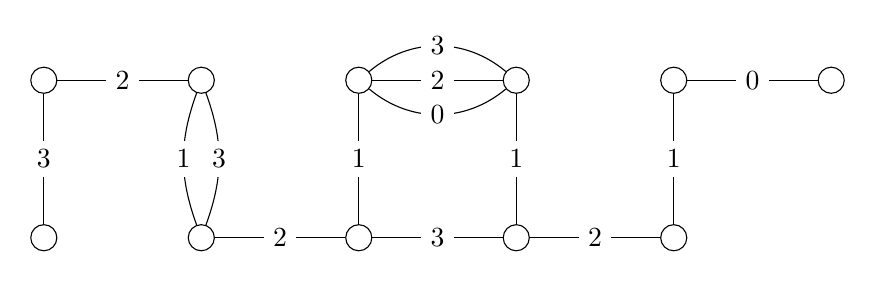
\begin{tikzpicture}

      \begin{scope}[every node/.style={circle,draw}]
        \node (1)  at (4,2)  {};
        \node (2)  at (6,2)  {};
        \node (3)  at (8,2)  {};
        \node (4)  at (10,2) {};
        \node (5)  at (0,0)  {};
        \node (6)  at (0,2)  {};
        \node (7)  at (6,0)  {};
        \node (8)  at (4,0)  {};
        \node (9)  at (2,0)  {};
        \node (10) at (2,2)  {};
        \node (11) at (8,0)  {};
      \end{scope}

      \begin{scope}[every node/.style={fill=white}]

        \begin{scope}[every edge/.style={draw}]
          \path (1)  edge[bend right=40] node {$0$} (2);
          \path (3)  edge node {$0$} (4);
          \path (1)  edge node {$1$} (8);
          \path (2)  edge node {$1$} (7);
          \path (3)  edge node {$1$} (11);
          \path (9)  edge[bend left=20] node {$1$} (10);
          \path (1)  edge node {$2$} (2);
          \path (6)  edge node {$2$} (10);
          \path (7)  edge node {$2$} (11);
          \path (8)  edge node {$2$} (9);
          \path (1)  edge[bend left=40] node {$3$} (2);
          \path (5)  edge node {$3$} (6);
          \path (7)  edge node {$3$} (8);
          \path (9)  edge[bend right=20] node {$3$} (10);
        \end{scope}
      \end{scope}

    \end{tikzpicture}
    \caption{[1, 1029, 5790, 994]}
  \end{center}
\end{figure}

\subsection{Longueur 3}

\begin{figure}[H]
  \begin{center}
    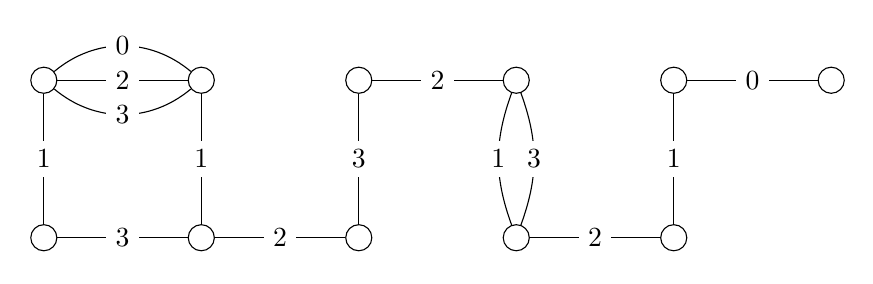
\begin{tikzpicture}

      \begin{scope}[every node/.style={circle,draw}]
        \node (1)  at (2,2)  {};
        \node (2)  at (0,2)  {};
        \node (3)  at (8,2)  {};
        \node (4)  at (10,2) {};
        \node (5)  at (4,2)  {};
        \node (6)  at (4,0)  {};
        \node (7)  at (0,0)  {};
        \node (8)  at (2,0)  {};
        \node (9)  at (6,2)  {};
        \node (10) at (6,0)  {};
        \node (11) at (8,0)  {};
      \end{scope}

      \begin{scope}[every node/.style={fill=white}]

        \begin{scope}[every edge/.style={draw}]
          \path (1)  edge[bend right=40] node {$0$} (2);
          \path (3)  edge node {$0$} (4);
          \path (1)  edge node {$1$} (8);
          \path (2)  edge node {$1$} (7);
          \path (3)  edge node {$1$} (11);
          \path (9)  edge[bend right=20] node {$1$} (10);
          \path (1)  edge node {$2$} (2);
          \path (5)  edge node {$2$} (9);
          \path (6)  edge node {$2$} (8);
          \path (10) edge node {$2$} (11);
          \path (1)  edge[bend left=40] node {$3$} (2);
          \path (5)  edge node {$3$} (6);
          \path (7)  edge node {$3$} (8);
          \path (9)  edge[bend left=20] node {$3$} (10);
        \end{scope}
      \end{scope}

    \end{tikzpicture}
    \caption{[1, 1029, 1584, 994]}
  \end{center}
\end{figure}

\begin{figure}[H]
  \begin{center}
    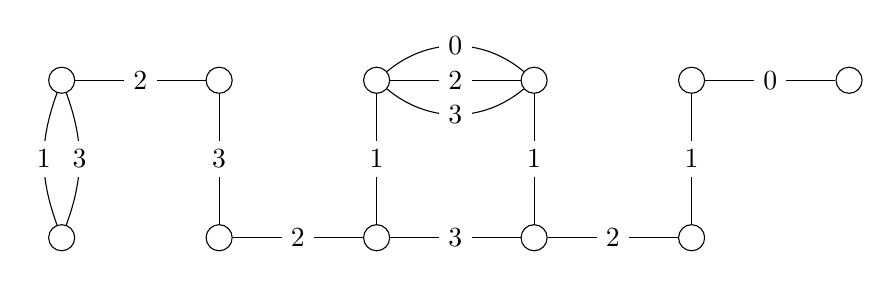
\begin{tikzpicture}

      \begin{scope}[every node/.style={circle,draw}]
        \node (1)  at (6,2)  {};
        \node (2)  at (4,2)  {};
        \node (3)  at (8,2)  {};
        \node (4)  at (10,2) {};
        \node (5)  at (2,2)  {};
        \node (6)  at (2,0)  {};
        \node (7)  at (4,0)  {};
        \node (8)  at (6,0)  {};
        \node (9)  at (0,2)  {};
        \node (10) at (0,0)  {};
        \node (11) at (8,0)  {};
      \end{scope}

      \begin{scope}[every node/.style={fill=white}]

        \begin{scope}[every edge/.style={draw}]
          \path (1)  edge[bend right=40] node {$0$} (2);
          \path (3)  edge node {$0$} (4);
          \path (1)  edge node {$1$} (8);
          \path (2)  edge node {$1$} (7);
          \path (3)  edge node {$1$} (11);
          \path (9)  edge[bend right=20] node {$1$} (10);
          \path (1)  edge node {$2$} (2);
          \path (5)  edge node {$2$} (9);
          \path (6)  edge node {$2$} (7);
          \path (8)  edge node {$2$} (11);
          \path (1)  edge[bend left=40] node {$3$} (2);
          \path (5)  edge node {$3$} (6);
          \path (7)  edge node {$3$} (8);
          \path (9)  edge[bend left=20] node {$3$} (10);
        \end{scope}
      \end{scope}

    \end{tikzpicture}
    \caption{[1, 1029, 8472, 994]}
  \end{center}
\end{figure}

\section{Quatre 4-transpositions}

\begin{figure}[H]
  \begin{center}
    \begin{tikzpicture}

      \begin{scope}[every node/.style={circle,draw}]
        \node (1)  at (6,0)  {};
        \node (2)  at (6,2)  {};
        \node (3)  at (4,2)  {};
        \node (4)  at (4,0)  {};
        \node (5)  at (4,-2) {};
        \node (6)  at (2,-2) {};
        \node (7)  at (2,0)  {};
        \node (8)  at (2,2)  {};
        \node (9)  at (10,2) {};
        \node (10) at (8,2) {};
        \node (11) at (8,0) {};
      \end{scope}

      \begin{scope}[every node/.style={fill=white}]

        \begin{scope}[every edge/.style={draw}]
          \path (1)  edge node {$0$} (2);
          \path (3)  edge node {$0$} (4);
          \path (5)  edge[bend right=40] node {$0$} (6);
          \path (7)  edge node {$0$} (8);
          \path (1)  edge node {$1$} (11);
          \path (3)  edge[bend right=20] node {$1$} (8);
          \path (4)  edge node {$1$} (5);
          \path (6)  edge node {$1$} (7);
          \path (1)  edge node {$2$} (4);
          \path (2)  edge node {$2$} (3);
          \path (5)  edge node {$2$} (6);
          \path (10) edge node {$2$} (11);
          \path (3)  edge[bend left=20] node {$3$} (8);
          \path (4)  edge node {$3$} (7);
          \path (5)  edge[bend left=40] node {$3$} (6);
          \path (9)  edge node {$3$} (10);
        \end{scope}
      \end{scope}

    \end{tikzpicture}
    \caption{[991, 1410, 1129, 4098]}
  \end{center}
\end{figure}
